\capitulo{6}{Trabajos relacionados}

El análisis del proceso de diseño en entornos de modelado tridimensional ha sido objeto de creciente interés en los últimos años, especialmente en disciplinas como la arquitectura, la ingeniería y la educación. Este interés se fundamenta en la posibilidad de registrar automáticamente las interacciones del usuario con herramientas digitales, generando datos que permiten estudiar el comportamiento de diseño desde una perspectiva objetiva y cuantificable.

Con el fin de estructurar el estado del arte, los trabajos analizados se agrupan en cuatro líneas principales: (1) análisis basado en \textit{event logs} y process mining, (2) estudios sobre comportamiento del diseñador, (3) entornos virtuales e inmersivos y (4) aplicaciones educativas del modelado 3D.

\section{Análisis del proceso de diseño mediante event logs}

Una de las líneas más relevantes es el uso de registros de eventos generados por herramientas de modelado 3D. Estos registros permiten capturar de forma automática las acciones realizadas por el usuario durante el proceso de diseño.

Gao et al. proponen una estructura de datos basada en grafos para modelar la relación entre comandos y objetos en el proceso de modelado \cite{gao2021}. Este enfoque permite analizar la secuencia de acciones y comprender la lógica subyacente del proceso de diseño. Posteriormente, Gao et al. amplían esta línea mediante técnicas de \textit{process mining}, demostrando que es posible identificar patrones de comportamiento y relacionarlos con la creatividad del diseño \cite{gao2023}.

De forma complementaria, Liu et al. aplican estos principios en contextos educativos, mostrando que los \textit{event logs} permiten reconstruir el proceso de diseño de los estudiantes y analizar su evolución \cite{liu2022}. Asimismo, Xie et al. utilizan análisis de series temporales sobre datos de CAD para evaluar el comportamiento del diseñador y detectar patrones iterativos en el proceso \cite{xie2014}.

\textbf{Limitación:} Estos trabajos se centran principalmente en el análisis posterior de los datos y en entornos específicos como BIM o CAD, sin proporcionar herramientas integradas en entornos generalistas que permitan la recopilación de datos en tiempo real.

\section{Estudios sobre comportamiento del diseñador}

Otra línea de investigación se centra en comprender cómo los diseñadores trabajan y cómo varía su comportamiento en función de su experiencia.

Chen et al. analizan las diferencias entre diseñadores expertos y novatos, evidenciando que existen variaciones en las estrategias utilizadas durante el proceso de diseño \cite{chen2022}. En la misma línea, Casakin y Levy proponen un marco para medir el comportamiento del diseñador experto, identificando factores clave como la descomposición del problema o el uso de pensamiento conceptual \cite{casakin2023}.

Por su parte, Welch y Lim muestran que los diseñadores novatos no siguen los modelos teóricos tradicionales, sino que adoptan procesos más iterativos y menos estructurados, basados en la experimentación \cite{welch}.

\textbf{Limitación:} Estos trabajos se basan principalmente en análisis teóricos o experimentales, con conjuntos de datos reducidos o métodos intrusivos (protocolos, observación), lo que limita su escalabilidad.

\section{Entornos virtuales e inmersivos}

El avance de tecnologías como la realidad virtual ha abierto nuevas posibilidades para el estudio del proceso de diseño.

Wang et al. presentan un análisis a gran escala del comportamiento de diseño en entornos VR, utilizando datos de interacción para modelar el proceso de diseño de forma automatizada \cite{wang2024}. De forma similar, Krassmann et al. analizan el comportamiento de los usuarios en entornos virtuales mediante técnicas de seguimiento y visualización \cite{krassmann2018}.

\textbf{Limitación:} Estos enfoques requieren entornos específicos (VR o mundos virtuales), lo que limita su aplicabilidad en herramientas de uso general como Blender.

\section{Aplicaciones educativas del modelado 3D}

El modelado 3D también ha sido ampliamente utilizado en contextos educativos.

Sosna et al. demuestran que el uso de herramientas de modelado 3D favorece el desarrollo de la creatividad en estudiantes \cite{sosna2025}. Asimismo, Koh et al. evidencian que el uso de simulaciones 3D mejora la motivación y el rendimiento académico \cite{koh2010}.

\textbf{Limitación:} Estos trabajos se centran en resultados educativos, pero no profundizan en la captura estructurada del proceso de diseño ni en su análisis técnico detallado.

\section{Comparación con el presente trabajo}

A partir del análisis realizado, se observa que los trabajos existentes presentan avances significativos en la comprensión del proceso de diseño, pero también importantes limitaciones.

\begin{itemize}
    \item La mayoría de estudios analizan datos \textbf{a posteriori}, en lugar de capturarlos en tiempo real.
    \item Muchos enfoques dependen de \textbf{entornos específicos} (BIM, VR, plataformas educativas).
    \item Existen limitaciones en la \textbf{integración directa con herramientas de modelado generalistas}.
    \item La captura de datos suele requerir \textbf{configuraciones complejas o métodos intrusivos}.
\end{itemize}

En este contexto, el presente trabajo propone un enfoque diferente basado en el desarrollo de un addon para Blender que permite:

\begin{itemize}
    \item Registrar automáticamente la interacción del usuario en tiempo real.
    \item Extraer variables internas del entorno (escena, geometría, modificadores, etc.).
    \item Almacenar los datos de forma estructurada e integrada en el propio archivo.
    \item Facilitar su posterior análisis sin alterar el flujo de trabajo del usuario.
\end{itemize}

\textbf{Contribución clave:} A diferencia de los trabajos existentes, esta propuesta se centra en la \textbf{recopilación no intrusiva de datos en un entorno de modelado generalista}, proporcionando una base sólida para el análisis del proceso de diseño en condiciones reales de uso.

De este modo, el sistema desarrollado contribuye a cubrir el vacío existente entre la captura de datos y su análisis, integrando ambas fases dentro del propio entorno de modelado.

\tablaSmall{Comparativa de trabajos relacionados}{l c c c c}{comparativa_estado_arte}
{ \multicolumn{1}{l}{Trabajo} & Tiempo real & Generalista & No intrusivo & Análisis \\}{
Gao et al. (2021) &  &  & X & X \\
Gao et al. (2023) &  &  & X & X \\
Liu et al. (2022) &  &  & X & X \\
Xie et al. (2014) &  &  & X & X \\
Chen et al. (2022) &  & X &  & X \\
Casakin et al. (2023) &  & X &  & X \\
Wang et al. (2024) &  &  &  & X \\
Krassmann et al. (2018) &  &  &  & X \\
Sosna et al. (2025) &  & X & X &  \\
Koh et al. (2010) &  & X & X &  \\
\textbf{Este trabajo} & \textbf{X} & \textbf{X} & \textbf{X} & \textbf{X} \\
}

\begin{figure}[H]
\centering
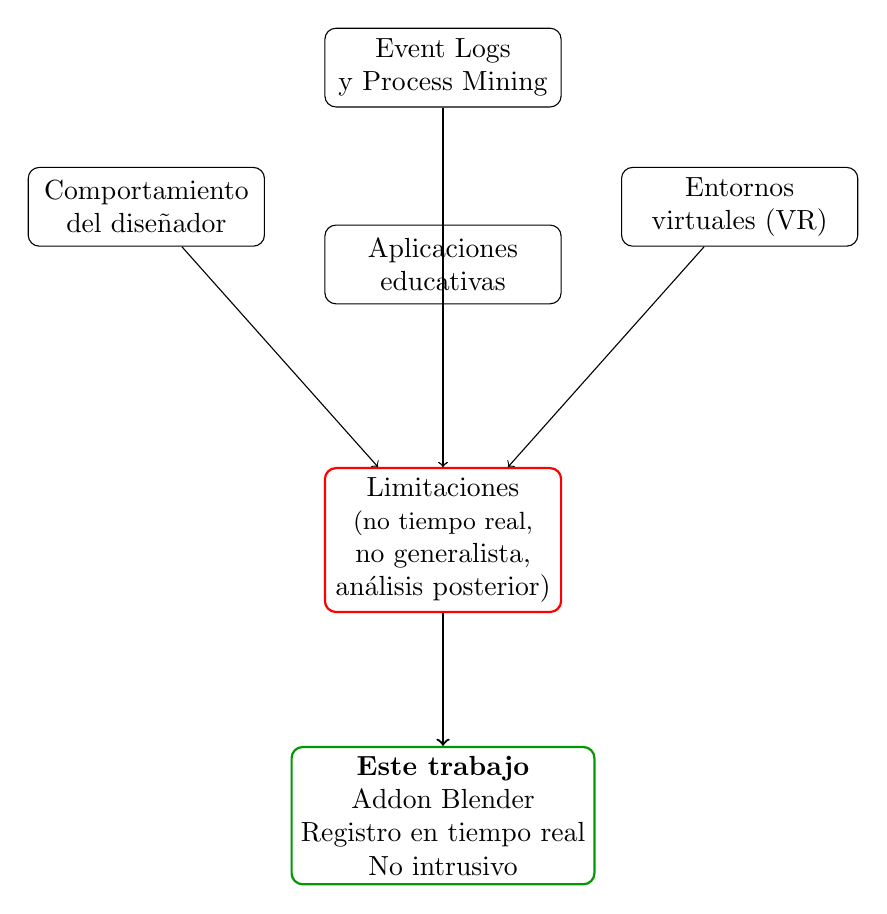
\begin{tikzpicture}[
    node distance=2.5cm,
    every node/.style={draw, rectangle, rounded corners, align=center, minimum width=3cm, minimum height=1cm}
]

\node (logs) {Event Logs \\ y Process Mining};
\node (behavior) [below left of=logs, xshift=-2cm] {Comportamiento \\ del diseñador};
\node (vr) [below right of=logs, xshift=2cm] {Entornos \\ virtuales (VR)};
\node (education) [below of=logs] {Aplicaciones \\ educativas};

\node (gap) [below of=education, yshift=-1cm, draw=red, thick] {Limitaciones \\ \small (no tiempo real, \\ no generalista, \\ análisis posterior)};

\node (solution) [below of=gap, yshift=-1cm, draw=green!60!black, thick] 
{\textbf{Este trabajo} \\ Addon Blender \\ Registro en tiempo real \\ No intrusivo};

\draw[->] (logs) -- (gap);
\draw[->] (behavior) -- (gap);
\draw[->] (vr) -- (gap);
\draw[->] (education) -- (gap);

\draw[->, thick] (gap) -- (solution);

\end{tikzpicture}
\caption{Resumen del estado del arte y posicionamiento del trabajo}
\end{figure}

En este contexto, la principal aportación de este trabajo consiste en el desarrollo de un sistema capaz de registrar de forma automática, estructurada y no intrusiva la interacción del usuario dentro de un entorno de modelado tridimensional generalista como Blender. 

A diferencia de los enfoques existentes, que se centran en el análisis posterior o en entornos específicos, esta propuesta permite capturar datos en tiempo real integrados en el flujo de trabajo del usuario, proporcionando una base sólida para el análisis del proceso de diseño en condiciones reales de uso.

El análisis de los trabajos relacionados pone de manifiesto la existencia de múltiples enfoques para el estudio del proceso de diseño, así como las limitaciones actuales en la recopilación de datos en entornos reales de modelado. 

En este contexto, el sistema desarrollado en este trabajo se posiciona como una solución que aborda estas limitaciones, integrando la captura de datos en tiempo real dentro del propio entorno de modelado. 

A continuación, se presentan las conclusiones obtenidas a partir del desarrollo y evaluación del sistema propuesto.

